\documentclass{article}

\usepackage{amsmath} % math stuff
\usepackage{amssymb} % math stuff
\usepackage{array} % equations and stuff
\usepackage{bm} % bold math
%\usepackage{booktabs} % extra table rule options
%\usepackage{caption} % suppressed table numbering; incompatible with revtex, and longtable, I think
\usepackage{comment} % comment environment
%\usepackage{enumitem} % customization of enumeration, itemize, and description
\usepackage[T1]{fontenc} % font encoding for special characters, must also use scalable font package
\usepackage[margin=0.8in]{geometry} % paper sizes and margins (but be careful not to mess up pre-defined pages)
\usepackage{graphicx} % for graphics
%\usepackage{helvet} % default font is the helvetica postscript font
\usepackage{layouts} % print units like widths
\usepackage{lipsum} % lorem ipsum filler text
\usepackage{lmodern} % scalable font?
\usepackage{longtable} % multi-page tables
\usepackage{makecell} % specify line-breaks in table cells
\usepackage{mathrsfs} % math script font
\usepackage{mhchem} % easier chemical formula
\usepackage{microtype} % allows disabling of ligatures
%\usepackage{newcent} % new century schoolbook font
\usepackage{nicefrac}
\usepackage{numprint} % print and format (large) numbers
\usepackage{parskip} % removes paragraph indentation, and adjusts paragraph skip, as well as list items
\usepackage{pdfpages} % add pdf files as pages
%\usepackage{setspace} % adjust text spacing and indents
\usepackage{siunitx} % decimal alignment
\usepackage{subfigure} % divided figures
%\usepackage{tabu} % extra table options
\usepackage{textcomp} % symbols
\usepackage{threeparttablex} % better footnotes with longtable
\usepackage{titling} % title placement
\usepackage{ulem} % strikethrough text
%\usepackage{url} % superceded by hyperref
\usepackage{verbatim} % verbatim environment
\usepackage{xcolor} % colors and color boxes
\usepackage{xspace} % commands that don't eat up white space
\usepackage{hyperref} % links and page setup; should always come last

\hypersetup{
 bookmarks=true,
 colorlinks=true,
 citecolor=blue,
 linkcolor=blue,
 urlcolor=blue,
 pdfstartview={XYZ null null 1.0} % default open view is 100%
}

\DisableLigatures[f,t]{encoding = T1} % disable ff, fi, fl, tt ligatures; without options, it also disables -- = endash
\renewcommand{\arraystretch}{1.0} % extra vertical (and horizontal?) space in tables

% define centered, left- and right-aligned columns with specified widths
\newcommand{\PreserveBackslash}[1]{\let\temp=\\#1\let\\=\temp}
\newcolumntype{C}[1]{>{\PreserveBackslash\centering}p{#1}}
\newcolumntype{L}[1]{>{\PreserveBackslash\raggedright}p{#1}}
\newcolumntype{R}[1]{>{\PreserveBackslash\raggedleft}p{#1}}

\begin{document}

\pagestyle{empty} % don't number pages

% custom title
\begin{center}
{\LARGE Express Riddler}

\vspace{0.15in}

{\Large 21 May 2021}
\end{center}


\section*{Riddle:}

The Riddler Cheese Company is producing what are called ``craft triples''---triangular slices of cheese whose side lengths are Pythagorean triples, when measured in inches.

However, the company's slicing machine recently malfunctioned and produced a stock of square slices with side lengths of 5 inches.
To salvage this situation, what is the greatest number of whole Pythagorean slices that can be made from each 5-inch square?
(Note: You can only cut pieces out of the square.
No melting or gluing pieces together!)

\textit{Extra credit}: What is the smallest square of cheese such that 100 percent of the square can be partitioned into craft triples?



\section*{Solution:}

My hand-drawn, not-to-scale solution is shown on the following page.
The $5\times5$ triangle can be divided into four 3-4-5 triangles.
Each triangle has a hypotenuse on an edge of the square, and there is a $1\times1$ square leftover in the center.
The triangles fit because the 3-5 and 4-5 angles of the triangle are complimentary.
Further, the area of each triangle is $\nicefrac{1}{2}*3*4=6$, so together they take up 24 of the 25 square inches of cheese.
The remaining 1 square inch is formed by the leftover lengths of sides: with each 3-inch side lined up against a 4-inch side leaves the 1 inch each time.
So the solution to the riddle is
\fcolorbox{red}{white}{\bf 4 triangles}.

For the extra credit, I believe that the answer is a 12-inch square.
This would be formed by doubling each 3-4-5 triangle, matching the hypotenuses to form $3\times4$ rectangles.
Arranging these $3\times4$ rectangles 4 across and 3 high would achieve a total length of 12 on each side.
I can't prove this is the answer, though.

\newpage

\begin{center}
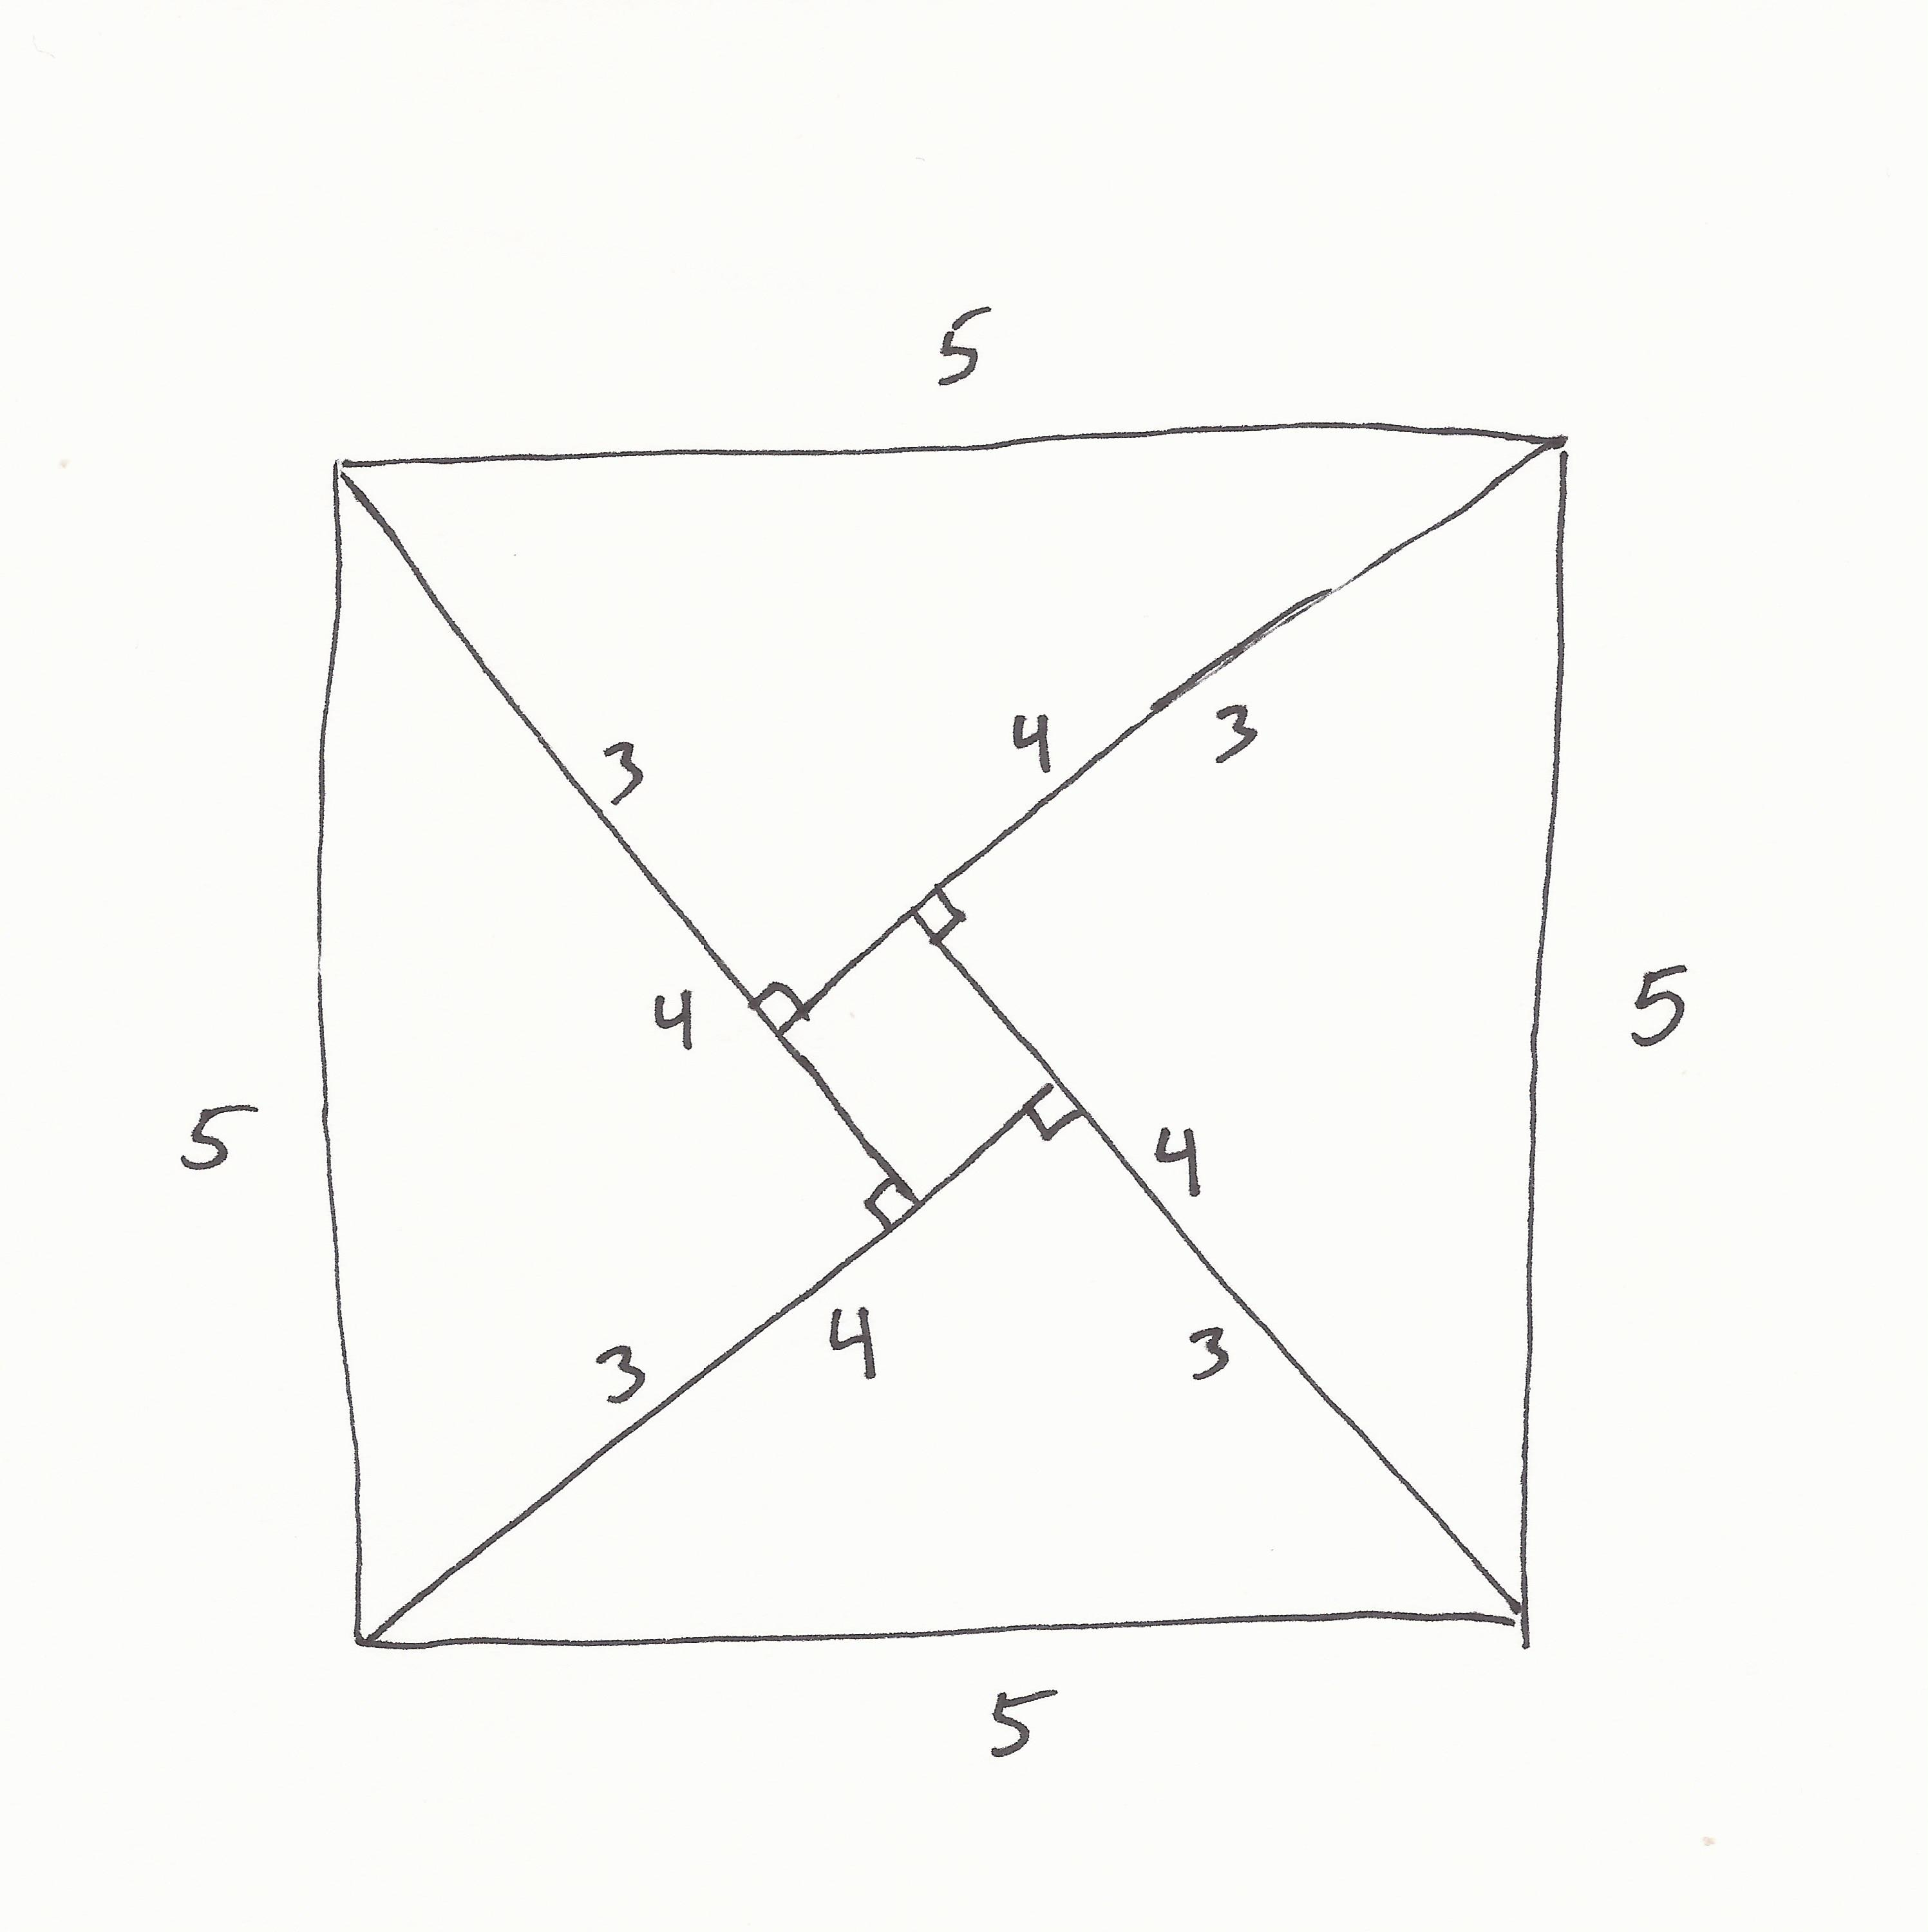
\includegraphics[width=5in]{Square_drawing.jpg}
\end{center}



\end{document}